\chapter{通信原理}

\section{数字频带传输}
        Modulation:用要传输的原始信号$m(t)$控制高频载波信号的某一参量,使它随$m(t)$发生变化。

        这个原始信号$m(t)$称为 \underline{调制信号}或 \underline{基带信号}。
        \begin{itemize}
            \item 模拟调制:$m(t)$为连续时间函数。
            \item 数字调制:调制信号为离散时间序列。
        \end{itemize}

        调制可以根据高频载波信号$C(t)$类型不同分类:
        \begin{itemize}
            \item 正弦波调制:正弦信号作为载波
            \item 脉冲调制:周期性脉冲作为载波
        \end{itemize}

        
        \begin{equation*}
        \mbox{根据调制参量来分类}
        \begin{cases}
            \mbox{正弦波模拟调制}\begin{cases}
                AM\\FM\\PM
            \end{cases}\\
            \mbox{正弦波数字调制}\begin{cases}
                ASK\\FSK\\PSK(相位键控)\\QAM(正交幅度调制)
            \end{cases}\\
            \mbox{脉冲模拟调制}\begin{cases}
                PAM\\PDM\\PPM
            \end{cases}\\
            \mbox{脉冲数字调制}\begin{cases}
                DPAM\\PCM\\DPCM\\ADPCM
            \end{cases}
        \end{cases}
        \end{equation*}


        \subsection{二进制通断键控(On-Off Keying)/二进制幅度键控(2ASK)}
            \begin{itemize}
                \item 传号时有一定幅度,空号时幅度为0。
                \item 可认为相位随机。
                \item 调制信号带宽是基带信号的2倍。
                \item 
            \end{itemize}
        
        \subsection{二进制相移键控(2PSK)}
            2PSK:用二进制数字基带信号控制正弦载波的相位。即码元的载波相位表示数字信息。

            设数字基带信号为双极性非归零信号$s(t)$,则2PSK信号调制过程
            \begin{equation}
                S_\mathrm{2PSK}(t)=s(t)\cos\omega_ct=
                \left\{\begin{aligned}
                    &A\cos(\omega_ct)\quad\mbox{“传号”}\\
                    -&A\cos(\omega_ct)\quad\mbox{“空号”}
                \end{aligned}\right.
                \qquad 0\leqslant t\leqslant T_b
            \end{equation}
            
        \begin{figure}[htp]
            \begin{center}
                \begin{tikzpicture}
                    [
                    node distance=6mm,
                    point/.style={circle,inner sep=0pt,minimum size=2pt,fill=black},
                    rect1/.style={shape = rectangle, draw ,text width = 1.2cm, align = flush center, minimum height = 1.2cm, inner sep=2mm},
                    ]
                    % % 辅助网格 标注原点
                    % \draw[step=1,help lines] (-5,-3) grid (5,3);
                    % \node [point] at (0,0) {};
                    % %
                    \node[label=below:{$S_\mathrm{2PSK}(t)$}] (in) {输入};
                    \node[rect1, right=of in] (信道) {信道};
                    \node[rect1, xshift=10mm, right=of 信道] (BPF) {BPF};
                    \node[draw, xshift=5mm, thick, circle, inner sep=-1pt, right=of BPF] (MUL) {\fontsize{20.74}{18}$\displaystyle \times$};
                    \node[rect1, right=of MUL] (LPF) {LPF};
                    \node[rect1, xshift=5mm, right=of LPF] (抽样判决器) {抽样\\判决器};
                    \node[xshift=5mm, label=below:{$P_e$}, right=of 抽样判决器] (out) {输出};

                    \node[below=of 信道] (噪声) {$n_i(t)$};
                    \node[below=of MUL, yshift=-4mm] (本振) {本地载波};
                    \node[below=of 抽样判决器] (定时脉冲) {定时脉冲};
                    %
                    \path[->,>=latex]
                        (in) edge node[] {} (信道)
                        (信道) edge node[below, pos=0.3] {$y_i(t)$} (BPF)
                        (BPF) edge node[below] {$y(t)$} (MUL)
                        (MUL) edge node[] {} (LPF)
                        (LPF) edge node[below] {$x(t)$} (抽样判决器)
                        (抽样判决器) edge node[] {} (out)

                        (噪声) edge (信道)
                        (本振) edge node [right, pos=0.4] {$2\cos\omega_c t$} (MUL)
                        (定时脉冲) edge (抽样判决器)
                    ;
                    \node [draw=black!50, dashed, very thick, rectangle, inner xsep = 4.7cm, inner ysep = 1.6cm, yshift=-0.4cm, xshift=1cm] at (MUL) {};
                \end{tikzpicture}
            \end{center}
            \caption{\kaishu 2PSK相干解调系统}\label{Fig: 2PSK相干解调系统}
        \end{figure}

        经过BPF,加性高斯白噪声变为窄带高斯噪声,有效信号的部分不变:
        \begin{equation}
            y(t)=
            \left\{\begin{aligned}{}
                [ &k_BA+n_c(t)]\cos\omega_ct-n_s(t)\sin\omega_ct\;,\; \mbox{"1"}\\
                [-&k_BA+n_c(t)]\cos\omega_ct-n_s(t)\sin\omega_ct\;,\; \mbox{"0"}
            \end{aligned}\right.
            \quad 0\leqslant t\leqslant T_b
        \end{equation}
        
        本振信号与BPF输出相乘(注意本振信号相位可能未对准),并经过LPF:
        \begin{equation}
            \begin{aligned}
                x(t)&=\mathrm{LPF}\left\{2[\pm k_BA+n_c(t)]\cos(\omega_ct)\cos(\omega_ct+\Delta\theta)-2n_s(t)\sin(\omega_ct)\cos(\omega_ct+\Delta\theta)\right\}\\
                &=\mathrm{LPF}\{2[\pm k_BA+n_c(t)][\cos^2(\omega_ct)\cos \Delta \theta-\cos(\omega_ct)\sin(\omega_ct)\sin \Delta \theta]\\
                                & \qquad \qquad -2n_s(t)[-\sin^2(\omega_ct)\sin \Delta \theta+\sin(\omega_ct)\cos\omega_ct\cos \Delta \theta]\}\\
                &=k_L[\pm k_BA+n_c(t)]\cos \Delta \theta +k_Ln_s(t)\sin \Delta \theta\\
            \end{aligned}
        \end{equation}
        
        理想情况下$\Delta \theta=0$,
        \begin{equation}
            x(t)=
            \left\{\begin{aligned}{}
                k_L [&k_BA+n_c(t)]\;,\quad \mbox{"1"}\\
                k_L[-&k_BA+n_c(t)]\;,\quad \mbox{"0"}
            \end{aligned}\right.
            \qquad 0\leqslant t\leqslant T_b
        \end{equation}
        
        最恶劣情况下$\Delta \theta=\pi$,
        \begin{equation}
            x(t)=
            \left\{\begin{aligned}{}
                k_L [-&k_BA-n_c(t)]\;,\quad \mbox{"1"}\\
                k_L[&k_BA-n_c(t)]\;,\quad \mbox{"0"}
            \end{aligned}\right.
            \qquad 0\leqslant t\leqslant T_b
        \end{equation}
        对于2PSK信号,这种情况导致解调系统反相工作。因此本地载波相位会导致输出绝对码反相,这种现象称为相位模糊。

        \subsection{二进制差分相移键控(2DPSK)}
        为解决2PSK信号存在的相位模糊问题,引入2DPSK。

        设数字基带信号为双极性非归零信号$s(t)$,对应的绝对码记作$\left\{a_n\right\}$,经过差分编码得到相对码$\left\{b_n\right\}$:
        \begin{equation}
            b_n=a_n\oplus b_{n-1}
        \end{equation}
        其中$\oplus$表示模二加,这里等价为异或运算。$\left\{b_n\right\}$的初始参考设为$0$。

        二进制下,相对码的“0”和“1”分别表示
        \begin{equation}
            b_n=
            \left\{\begin{aligned}
                &0\;,\quad \varphi_n-\varphi_{n-1}=0\\
                &1\;,\quad \varphi_n-\varphi_{n-1}=\pm \pi
            \end{aligned}\right.
        \end{equation}

        反过来由相对码得出绝对码的过程称为差分译码:
        \begin{equation}
            a_n=b_n\oplus b_{n-1}
        \end{equation}

        \begin{figure}[htp]
            \begin{center}
                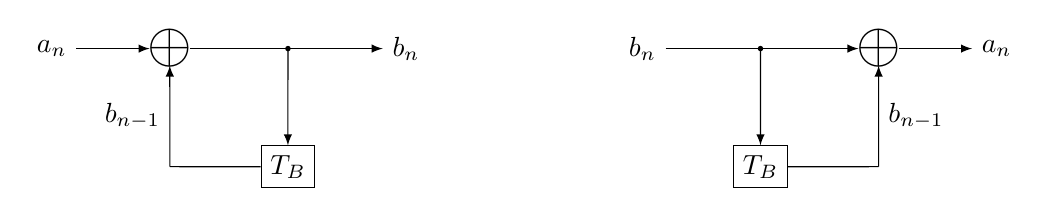
\begin{tikzpicture}[scale=1.5,
                    point/.style={circle,inner sep=0pt,minimum size=2pt,fill=black},]
                    % % 辅助网格 标注原点
                    % \draw[step=1,help lines] (-4,-2) grid (4,2);
                    % \node [point] at (0,0) {};
                    %
                    \coordinate (s) at (-3,0);
                    \coordinate (z) at (2,0);


                    % 差分编码
                    \draw (s)++(-2,0) node (A) {$a_n$};
                    \draw (s)++(-1,0) node[inner sep=-1pt] (S){\fontsize{20.74}{18}$\oplus$};
                    \draw (s)++(0,-1) node[draw] (D) {$T_B$};
                    \draw (s)++(1,0) node (B) {$b_n$};
                    %
                    \path[->,>=latex]
                        (A) edge (S)
                        (S) edge (B)
                        (s) edge (D)
                    ;
                    \node [point] at (s) {};
                    \draw (s)++(-1,-1) -- (D.west)
                        (s)++(-1,-1) edge[->,>=latex] node[left] {$b_{n-1}$} (S.south) ;
                    % 差分译码
                    \draw (z)++(-2,0) node (A) {$b_n$};
                    \draw (z)++(-1,-1) node[draw] (D) {$T_B$};
                    \draw (z)++(0,0) node[inner sep=-1pt] (S){\fontsize{20.74}{18}$\oplus$};
                    \draw (z)++(1,0) node (B) {$a_n$};
                    %
                    \path[->,>=latex]
                        (A) edge (S)
                        (S) edge (B)
                        (z)++(-1,0) edge (D)
                    ;
                    \draw (z)++(-1,0) node[point]  {};
                    \draw (z)++(0,-1) -- (D.east)
                        (z)++(0,-1) edge[->,>=latex] node[right] {$b_{n-1}$} (S.south) ;

                \end{tikzpicture}
            \end{center}
            \caption{\kaishu 差分译码和差分解码}\label{Fig: 差分译码和差分解码}
        \end{figure}

        绝对码$\left\{a_n\right\}$的2DPSK信号,就是相对码$\left\{b_n\right\}$的2PSK信号。即经过差分译码后,可通过产生PSK信号的方式产生DPSK信号。

        2DPSK信号的解调可以使用相干解调加差分译码的方式,也可以用差分相干解调法
        \begin{figure}[htp]
            \begin{center}\resizebox{\textwidth}{!}{
                \begin{tikzpicture}
                    [
                    node distance=6mm,
                    point/.style={circle,inner sep=0pt,minimum size=2pt,fill=black},
                    rect1/.style={shape = rectangle, draw ,text width = 1.2cm, align = flush center, minimum height = 1.2cm, inner sep=2mm},
                    ]
                    % % 辅助网格 标注原点
                    % \draw[step=1,help lines] (-5,-3) grid (5,3);
                    % \node [point] at (0,0) {};
                    % %
                    \node[label=below:{$S_\mathrm{2DPSK}(t)$}] (in) {输入};
                    \node[rect1, right=of in] (信道) {信道};
                    \node[rect1, xshift=10mm, right=of 信道] (BPF) {BPF};
                    \node[draw, xshift=5mm, thick, circle, inner sep=-1pt, right=of BPF] (MUL) {\fontsize{20.74}{18}$\displaystyle \times$};
                    \node[rect1, right=of MUL] (LPF) {LPF};
                    \node[rect1, xshift=5mm, right=of LPF] (抽样判决器) {抽样\\判决器};
                    \node[rect1, xshift=7mm, right=of 抽样判决器] (差分译码) {差分\\译码};
                    \node[xshift=5mm, label=below:{$a_n$}, right=of 差分译码] (out) {输出};

                    \node[below=of 信道] (噪声) {$n_i(t)$};
                    \node[below=of MUL, yshift=-4mm] (本振) {本地载波};
                    \node[below=of 抽样判决器] (定时脉冲) {定时脉冲};
                    %
                    \path[->,>=latex]
                        (in) edge node[] {} (信道)
                        (信道) edge node[below, pos=0.3] {$y_i(t)$} (BPF)
                        (BPF) edge node[below] {$y(t)$} (MUL)
                        (MUL) edge node[] {} (LPF)
                        (LPF) edge node[below] {$x(t)$} (抽样判决器)
                        (抽样判决器) edge node[below, pos=0.7] {$b_n$} (差分译码)
                        (差分译码) edge node[] {} (out)

                        (噪声) edge (信道)
                        (本振) edge node [right, pos=0.4] {$2\cos\omega_c t$} (MUL)
                        (定时脉冲) edge (抽样判决器)
                    ;
                    \node [draw=black!50, dashed, very thick, rectangle, inner xsep = 4.7cm, inner ysep = 1.6cm, yshift=-0.4cm, xshift=1cm] at (MUL) {};
                \end{tikzpicture}}
            \end{center}
            \caption{\kaishu 2DPSK相干解调系统}\label{Fig: 2DPSK相干解调系统}
        \end{figure}

        相干解调部分和PSK解调相同,若只考虑一个码元内的波形:

    \section{移动通讯}
    \subsection{5G}

    \subsection{6G}

    覆盖率(到90\%)、传输速度(Tbps)、低延时(1ms)、定位精度、可靠性、低功耗、智能水平。

    
    